\chapter{Creating a Repository (Stratum~0)}
\label{sct:createrepo}

% Introduction
% Components
% Installation / Requirements
% Cvmfs server and cvmfs swissknife

\cvmfs\ is a file system with a single source of (new) data.
This single source, the repository \emph{Stratum 0}, is maintained by a dedicated \emph{release manager machine} or \emph{installation box}.
A read-writable copy of the repository is accessible on the release manager machine.
The \cvmfs\ server tool kit is used to \emph{publish} the current state of the repository on the release manager machine.
Publishing is an atomic operation.

All data stored in \cvmfs\ have to be converted into a \cvmfs\ \emph{repository} during the process of publishing.
The \cvmfs\ repository is a form of content-addressable storage.
Conversion includes creating the file catalog(s), compressing new and updated files and calculating content hashes.
Storing the data in a content-addressable format results in automatic file de-duplication.
It furthermore simplifies data verification and it allows for file system snapshots.

In order to provide a writable \cvmfs\ repository, \cvmfs\ uses a union file system that combines a read-only \cvmfs\ mount point with a writable scratch area~\cite{unionfs04,aufs}.
Figure~\ref{fig:installwebserver} outlines the process of publishing a repository.

\begin{figure}[h]
	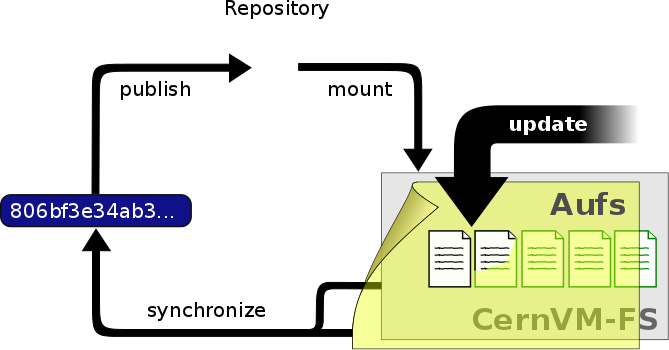
\includegraphics[width=\textwidth]{figures/update_process.png}
	\caption{Updating a mounted \cvmfs\ repository by overlaying it with a copy-on-write \aufs\ volume. 
		Any changes will be accumulated in a writable volume (yellow) and can be synchronized into the \cvmfs\ repository afterwards. 
		The file catalog contains the directory structure as well as file metadata, symbolic links, and secure hash keys of regular files. 
		Regular files are compressed and renamed to their cryptographic content hash before copied into the data store.}
	\label{fig:installwebserver}
\end{figure}

\section{Publishing a new Repository Revision}
\label{sct:repoupdate}

Since the repositories may contain many file system objects\footnote{For ATLAS, for example, ``many'' means order of $10^7$ file system objects (\ie number of regular files, symbolic links, and directories).}, we cannot afford to generate an entire repository from scratch for every update.
Instead, we add a writable file system layer on top of a mounted read-only \cvmfs\ repository using the union file system \aufs~\cite{aufs}.
This renders a read-only \cvmfs\ mount point writable to the user, while all performed changes are stored in a special writable scratch area managed by \aufs.
A similar approach is used by Linux Live Distributions that are shipped on read-only media, but allow \emph{virtual} editing of files where changes are stored on a RAM disk.

If a file in the \cvmfs\ repository gets changed, \aufs\ first copies it to the writable volume and applies any changes to this copy (copy-on-write semantics).
\aufs\ will put newly created files or directories in the writable volume as well.
Additionally it creates special hidden files (called \emph{white-outs}) to keep track of file deletions in the \cvmfs\ repository.

Eventually, all changes applied to the repository are stored in \aufs's scratch area and can be merged into the actual \cvmfs\ repository by a subsequent synchronization step.
Before the actual synchronization step takes place, no changes are applied to the \cvmfs\ repository.
Therefore, any unsuccessful updates to a repository can be rolled back by simply clearing the writable file system layer of \aufs.

\section{Requirements for a new Repository}
\label{sct:newreporequirements}

In order to create a repository, the server and client part of \cvmfs\ must be installed on the release manager machine.
Furthermore your machine should provide an \aufs\ enabled Kernel as well as a running \texttt{Apache2} web server.
Currently we support Scientific Linux 6 and Ubuntu 12.04 distributions.
Please note, that Scientific Linux 6 \emph{does not} ship with an \aufs\ enabled kernel, therefore we provide a compatible patched kernel as RPMs (see Appendix~\ref{apx:rpms}).


\section{\cvmfs\ Repository Creation and Updating}
\label{sct:repocreateandupdate}
The \cvmfs\ server tool kit provide the versatile \texttt{cvmfs\_server} utility in order to perform all operations related to repository creation, updating, deletion, replication and inspection.
Please run it without any parameters to get a short documentation of its commands.

\subsection{Repository Creation}
\label{sct:repocreation}

A new repository is created by \texttt{cvmfs\_server mkfs}:
\begin{verbatim}
  cvmfs_server mkfs my.repo.name
\end{verbatim}
The utility will then ask you for a user that should act as the owner of the repository and afterwards create all the infrastructure for the new \cvmfs\ repository.
Additionally it will create a reasonable default configuration and generate a new release manager certificate and software signing key. 
You'll have to distribute the public key in /etc/cvmfs/keys/my.repo.name.pub to all your client machines.
The \texttt{cvmfs\_server} utility will use \texttt{/srv/cvmfs} as storage location.
In case you want to use a separate hard disk, you should mount it there upfront.

Once created, you should see your repository mounted under \texttt{/cvmfs/my.repo.name} containing only a single file called \texttt{new\_repository}.
Following this step, you can produce the first revision by going through the repository update procedure described in the next section.

\subsubsection{Repositories for Volatile Files}
Repositories can be flagged as containing \emph{volatile} files using the \texttt{-v} option:
\begin{verbatim}
  cvmfs_server mkfs -v my.repo.name
\end{verbatim}
When \cvmfs\ clients perform a cache cleanup, they treat files from volatile repositories with priority.
Such volatile repositories can be useful, for instance, for experiment conditions data.

\subsection{Repository Update}
\label{sct:repoupdateprocedure}
Typically a repository publisher does the following steps in order to create a new revision of a repository:
\begin{enumerate}
	\item Run \texttt{cvmfs\_server transaction} to switch to a copy-on-write enabled \cvmfs\ volume
	\item Make the necessary changes to the repository, \eg add new directories, patch certain binaries, \dots
	\item Test the software installation
	\item Do one of the following:
	\begin{itemize}
		\item Run \texttt{cvmfs\_server publish} to finalize your new repository revision \emph{or}
		\item Run \texttt{cvmfs\_server abort} to clear all changes and start over again
	\end{itemize}
	\item Make the web server serve the new version of the repository directory.
\end{enumerate}

\cvmfs\ supports to have more than one repository on a single server machine.
In case of a multi-repository host, you need to specify which repository you want to operate on, when running the \texttt{cvmfs\_server} utility commands.
Additionally you should run \texttt{cvmfs\_server resign} every 30 days to update the signatures of the repository.
Most \texttt{cvmfs\_server} commands allow for wildcards to do manipulations on more than one repository at once, i.e. \texttt{cvmfs\_server migrate *.cern.ch} would migrate all present repositories ending with \texttt{.cern.ch}.

\subsection{Repository Import}
The \cvmfs\ 2.1 server tools support the import of a \cvmfs\ file storage together with its corresponding signing keychain.
With \texttt{cvmfs\_server import} both \cvmfs\ 2.0 and 2.1 compliant repository file storages can be imported.

\texttt{cvmfs\_server import} works similar to \texttt{cvmfs\_server mkfs} (see \ref{sct:repocreation}) except it uses the provided data storage instead of creating a fresh (and empty) storage.
In case of a \cvmfs\ 2.0 file storage \texttt{cvmfs\_server import} also takes care of the file catalog migration into the \cvmfs\ 2.1 schema.

\subsubsection{Legacy Repository Import}
We strongly recommend to install \cvmfs\ 2.1 on a fresh or at least a properly cleaned  machine without any traces of the \cvmfs\ 2.0 installation before installing \cvmfs\ 2.1 server tools.

The command \texttt{cvmfs\_server import} requires the full \cvmfs\ 2.0 data storage which is located at /srv/cvmfs by default as well as the repository's signing keys.
Since the \cvmfs\ 2.1 server backend supports multiple repositories in contrast to its 2.0 counterpart, we recommend to move the repository's data storage to /srv/cvmfs/<FQRN> upfront to avoid later inconsistencies.

\vspace*\baselineskip
In order to transform a repository from \cvmfs\ 2.0 into 2.1 you should roughly follow the following steps. As an example we are using a repository called \textbf{legacy.cern.ch}.
\begin{enumerate}
	\item Make sure that you have backups of both the repository's backend storage and its signing keys
	\item Install and test the \cvmfs\ 2.1 server tools on the machine you are going to use as your Stratum 0 maintenance machine
	\item Place the repository's backend storage data in /srv/cvmfs/\textit{legacy.cern.ch} \\ (default storage location)
	\item Transfer the repository's signing keychain to the machine (f.e. to \textapprox/legacy\_keys/)
	\item Run \texttt{cvmfs\_server import} roughly like this:
\begin{verbatim}
    cvmfs_server import
      -o <username of repo maintainer> \
      -k ~/legacy_keys \
      -l               \ # for 2.0.x file catalog migration
      -s               \ # for further repository statistics
      legacy.cern.ch
\end{verbatim}
    \item Check the imported repository with \texttt{cvmfs\_server check legacy.cern.ch} for integrity (see \ref{sct:checkintegrity})
\end{enumerate}


\subsection{Customizable Actions Using Server Hooks}
The \texttt{cvmfs\_server} utility allows release managers to trigger custom actions before and after crucial repository manipulation steps. This can be useful for example for logging purposes, establishing backend storage connections automatically or other workflow triggers, depending on the application.

There are six designated server hooks that are potentially invoked during the repository update procedure described in Section \ref{sct:repoupdateprocedure}:
\begin{itemize}
	\item When running \texttt{cvmfs\_server transaction}:
	\begin{itemize}
		\item \emph{before} the given repository is transitioned into transaction mode
		\item \emph{after} the transition was successful
	\end{itemize}
	\item When running \texttt{cvmfs\_server publish}:
	\begin{itemize}
		\item \emph{before} the publish procedure for the given repository is started
		\item \emph{after} it was published and remounted successfully
	\end{itemize}
	\item When running \texttt{cvmfs\_server abort}:
	\begin{itemize}
		\item \emph{before} the unpublished changes will be erased for the given repository
		\item \emph{after} the repository was successfully reverted to the last published state
	\end{itemize}
\end{itemize}
All server hooks must be defined in a single shell script file called:
\begin{verbatim}
/etc/cvmfs/cvmfs_server_hooks.sh
\end{verbatim}
The \texttt{cvmfs\_server} utility will check the existence of this script and source it.
To subscribe to the described hooks one needs to define one or more of the following shell script functions:
\begin{itemize}
	\setlength{\itemsep}{1pt}
	\item \texttt{transaction\_before\_hook()}
	\item \texttt{transaction\_after\_hook()}
\end{itemize}
\begin{itemize}
	\item \texttt{publish\_before\_hook()}
	\item \texttt{publish\_after\_hook()}
\end{itemize}
\begin{itemize}
	\item \texttt{abort\_before\_hook()}
	\item \texttt{abort\_after\_hook()}
\end{itemize}
The defined functions get called at the specified positions in the repository update process and are provided with the fully qualified repository name as their only parameter~(\texttt{\$1}).
Undefined functions automatically default to a NO-OP.
You might consult the example script located at \texttt{cvmfs/cvmfs\_server\_hooks.sh.demo} in the \cvmfs\ sources.


\section{Maintaining a CernVM-FS Repository}

\cvmfs\ is a versioning, snapshot-based file system. 
Similar to versioning systems, changes to /cvmfs/\dots are temporary until they are committed (\texttt{cvmfs\_server publish}) or discarded (\texttt{cvmfs\_server abort}). 
That allows you to test and verify your changes, for instance to test a newly installed release before publishing it to clients.
Whenever changes are published (committed), a new file system snapshot of the current state is created. 
These file system snapshots can be tagged with a name, which makes them \emph{named snapshots}. 
A named snapshot is meant to stay in the file system. 
You can rollback to named snapshots and you can, on client side, decide to mount any of the named snapshots in lieu of the newest available snapshot.

Two named snapshots are managed automatically by \cvmfs, \texttt{trunk} and \texttt{trunk-previous}. 
This allows for easy unpublishing of a mistake, by rolling back to the \texttt{trunk-previous} tag.

\subsection{Check Integrity}
\label{sct:checkintegrity}
\cvmfs\ provides an integrity checker for repositories.
Run the integrity checker using
\begin{verbatim}
cvmfs_server check
\end{verbatim}

The integrity checker verifies the sanity of file catalogs and verifies that referenced data chunks are present.
Ideally, run the integrity checker after every publish operation.
Where this is not affordable due to the size of the repositories, run the integrity checker regularly.

Optionally \texttt{cvmfs\_server check} can also verify the data integrity (command line flag \texttt{-i}) of each data object in the repository.
However this is a time consuming process and we recommend it only for diagnostic purposes.

\subsection{Manage Named Snapshots}

At the point of publishing, the resulting snapshot can be named. 
To do so, use the -a option like
\begin{verbatim}
cvmfs_server transaction
# Changes
cvmfs_server publish -a release-1.0
\end{verbatim}

As a tag name, use an identifier without spaces and special characters. 
You can list all named snapshots by 
\begin{verbatim}
cvmfs_server lstags
\end{verbatim}

In order to remove (unpublish) a named snapshot, use the -r option like
\begin{verbatim}
cvmfs_server transaction
cvmfs_server publish -r release-1.0
\end{verbatim}

Use named snapshots whenever you do larger modifications to the repository, for instance when you install a new software release. 
Only with named snapshots you have the ability to easily undo modifications and to preserve the state of the file system for the future. 
Nevertheless, do not use named snapshots excessively. 
Start cleaning up unneccesary snapshots once you have more than $\approx 50$.

\subsection{Rollbacks}

You can rollback your repository to any of the named snapshots. 
Technically, this means that the given snapshot is re-published, while all intermediate snapshots are removed from the history.

In order to rollback, do
\begin{verbatim}
cvmfs_server transaction
cvmfs_server rollback -t release-1.0
\end{verbatim}

A rollback is, like restoring from backups, not something you would do often. 
Use caution. 
A rollback is irreversible.

\subsection{Manage Nested Catalogs}

\cvmfs\ stores meta-data (path names, file sizes, \dots) in file catalogs. 
When a client accesses a repository, it has to download the file catalog first and then it downloads the files as they are opened. 
A single file catalog for an entire repository can quickly become large and impractical. 
At the same time, clients typically do not need all of the repository's meta-data at the same time. 
For instance, clients using software release 1.0 do not need to know about the contents of software release 2.0.

With nested catalogs, \cvmfs\ has a mechansim to partition the directory tree of a repository into many catalogs. 
Repository maintainers are responsible for sensible cutting of the directory trees into nested catalogs. 
They can do so by creating and removing the magic file \texttt{.cvmfscatalog}.

For example, in order to create a nested catalog for software release 1.0 in the hypothetical repository experiment.cern.ch, do
\begin{verbatim}
cvmfs_transaction
touch /cvmfs/experiment.cern.ch/software/1.0/.cvmfscatalog
cvmfs_server publish
\end{verbatim}

If you want to merge a nested catalog with its parent catalog, remove the corresponding \texttt{.cvmfscatalog} file. 
Nested catalogs can be nested on arbitrary many levels.

\subsection{Recommendations for Nested Catalogs}
Nested catalogs should be created having in mind which files and directories are accessed together. 
This is typically the case for software releases, but can be also on the directory level that separates platforms. 
For instance, for a directory layout like
\begin{verbatim}
/cvmfs/experiment.cern.ch
  |- /software
  |    |- /i686
  |    |    |- 1.0
  |    |    |- 2.0
  |    `    |- common
  |    |- /x86_64
  |    |    |- 1.0
  |    `    |- common  
  |- /grid-certificates
  |- /scripts 
\end{verbatim}
it makes sense to have nested catalogs at
\begin{verbatim}
/cvmfs/experiment.cern.ch/software/i686
/cvmfs/experiment.cern.ch/software/x86_64
/cvmfs/experiment.cern.ch/software/i686/1.0
/cvmfs/experiment.cern.ch/software/i686/2.0
/cvmfs/experiment.cern.ch/software/x86_64/1.0 
\end{verbatim}

It could also make sense to have a nested catalog under grid-certificates, if the certificates are updated much more frequently than the other directories. 
It would not make sense to create a nested catalog under /cvmfs/experiment.cern.ch/software/i686/common, because this directory needs to be accessed anyway whenever its parent directory is needed.
As a rule of thumb, a single file catalog should contain more than 1000 files and directories but not contain more than ~200\,000 files.

Restructuring the repository's directory tree is an expensive operation in CernVM-FS. 
Moreover, it can easily break clients when they switch to a restructured file system snapshot. 
Therefore, your software directory tree layout should be relatively stable before you start filling the CernVM-FS repository.

\subsection{Migrate File Catalogs}
In rare cases the further development of \cvmfs\ makes it necessary to change the internal structure of file catalogs.
Updating the \cvmfs\ installation on a Stratum 0 machine might require a migration of the file catalogs.

It is recommended that \texttt{cvmfs\_server list} is issued after any \cvmfs\ update to review if any of the maintained repositories need a migration.
Outdated repositories will be marked as \textbf{INCOMPATIBLE} and \texttt{cvmfs\_server} refuses all actions on these repositories until the file catalogs have been updated.

In order to run a file catalog migration use \texttt{cvmfs\_server migrate} for each of the outdated repositories.
This will essentially create a new repository revision that contains the exact same  file structure as the current revision.
However, all file catalogs will be recreated from scratch using the updated internal structure.
Note that historic file catalogs of all previous repository revisions stay untouched and are not migrated.

After \texttt{cvmfs\_server migrate} has successfully updated all file catalogs repository maintenance can continue as usual.
